\documentclass{beamer}
\usepackage[utf8]{inputenc}
\usepackage{listings}
\usetheme{Warsaw}
\title[Android: Diseño de la capa red]{Diseño de sistemas de información\\Capa de red en Android}
\author{Santiago Munín}
\institute{Universidade da Coruña}
\date{Mayo, 2013}
\begin{document}

\begin{frame}
\titlepage
\end{frame}

\section{Introducción}
\begin{frame}{Motivación}
\begin{itemize}
\item Gran parte de las aplicaciones móviles de éxito emplean una aquitectura Cliente/Servidor.
\item Estas arquitecturas utilizan la red como medio para comunicarse.
\item {\bf Ejemplos}: Twitter, Facebook, 4square, Evernote...
\end{itemize}
\end{frame}

\begin{frame}{Arquitectura Cliente/Servidor}
\begin{itemize}
\item La comunicación suele realizarse mediante HTTP (o HTTPS) contra servidores (habitualmente REST).
\item Se emplean tecnologías como JSON o XML para transmitir información.
\item Esta comunicación es potencialmente costosa $\rightarrow$ Si se realiza en el thread de la interfaz (thread principal) puede bloquear demasiado tiempo el teléfono y afectar a la experiencia del usuario.
\item La solución a este problema es sencilla: ejecutar en segundo plano la petición y actualizar la interfaz una vez recibiba la respuesta (mientras tanto, permitir al usuario interactuar con la aplicación o mostrar un diálogo de carga).
\end{itemize}
\end{frame}

\begin{frame}{AsyncTask}
\begin{itemize}
\item Android nos ofrece una clase que encapsula el manejo de threads.
\item AsyncTask nos permite ejecutar una tarea en segundo plano y usar el resultado de la misma en primer plano (una vez haya acabado) sin bloquear la interfaz.
\item {\bf Más información}: \url{http://developer.android.com/reference/android/os/AsyncTask.html}
\end{itemize}
\end{frame}

\section{Primer diseño: solución ``directa''}
\subsection{Diagrama de clases}
\begin{frame}{Diagrama de clases}
\begin{figure}
\begin{center}
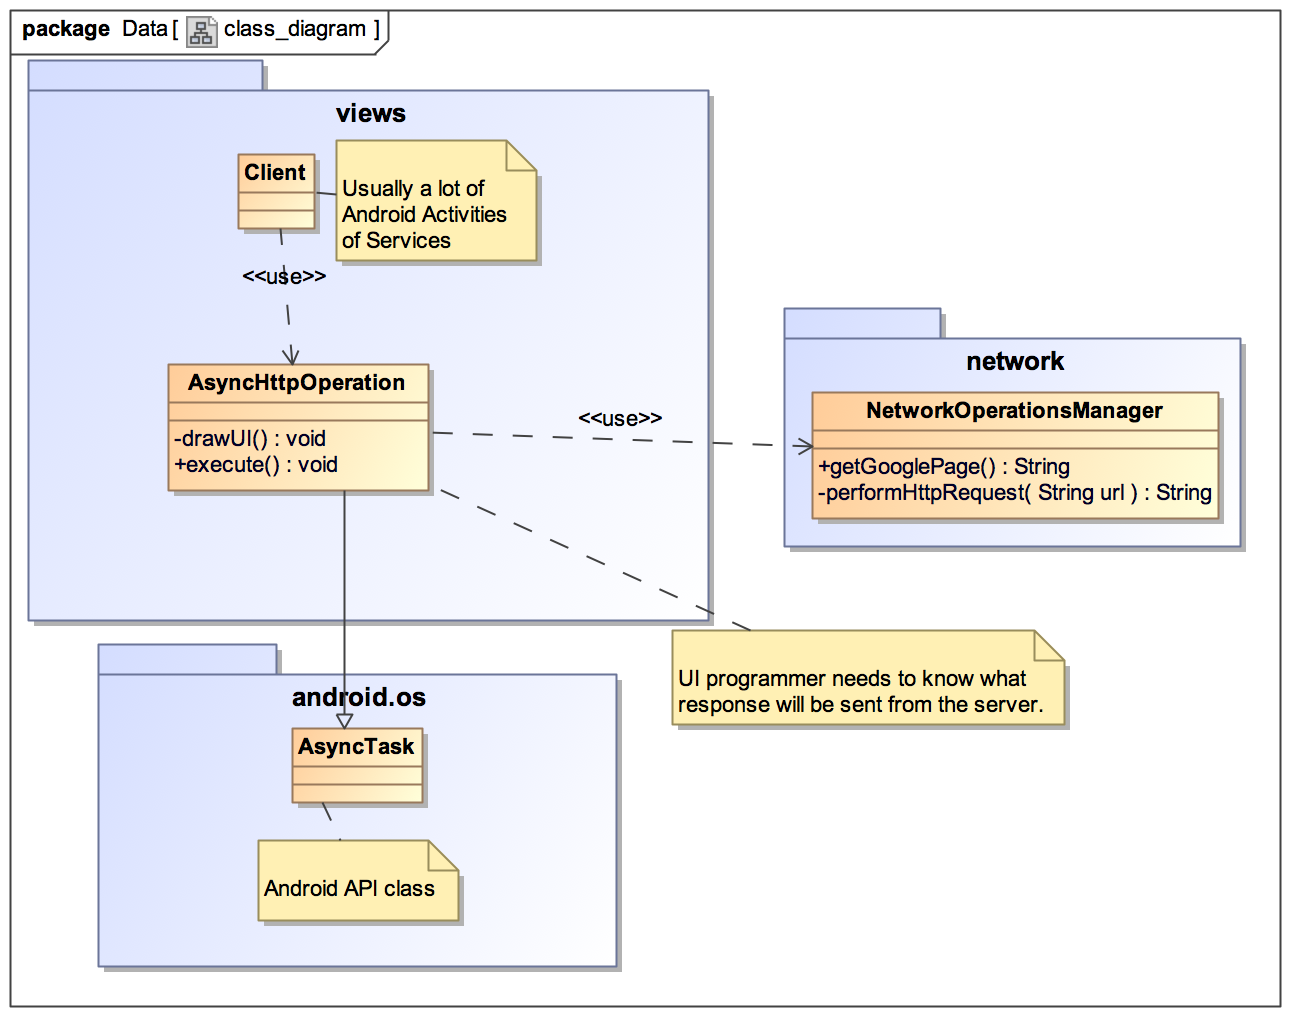
\includegraphics[scale=0.6]{../naive/design_models/class_diagram}
\end{center}
\end{figure}
\end{frame}

\begin{frame}{Explicación}
\begin{itemize}
\item El cliente (habitualmente ``Activities'' Android) utiliza clases que heredan de ``AsyncTask'' para no bloquear la interfaz.
\item La clase ``NetworkOperationsManager'' contiene la lógica relacionada con las llamadas en red (direcciones, parámetros...). Podría ser responsable del cacheo de respuestas.
\end{itemize}
\end{frame}

\subsection{Diagrama de secuencia}
\begin{frame}{Diagrama de secuencia}
\begin{figure}
\begin{center}
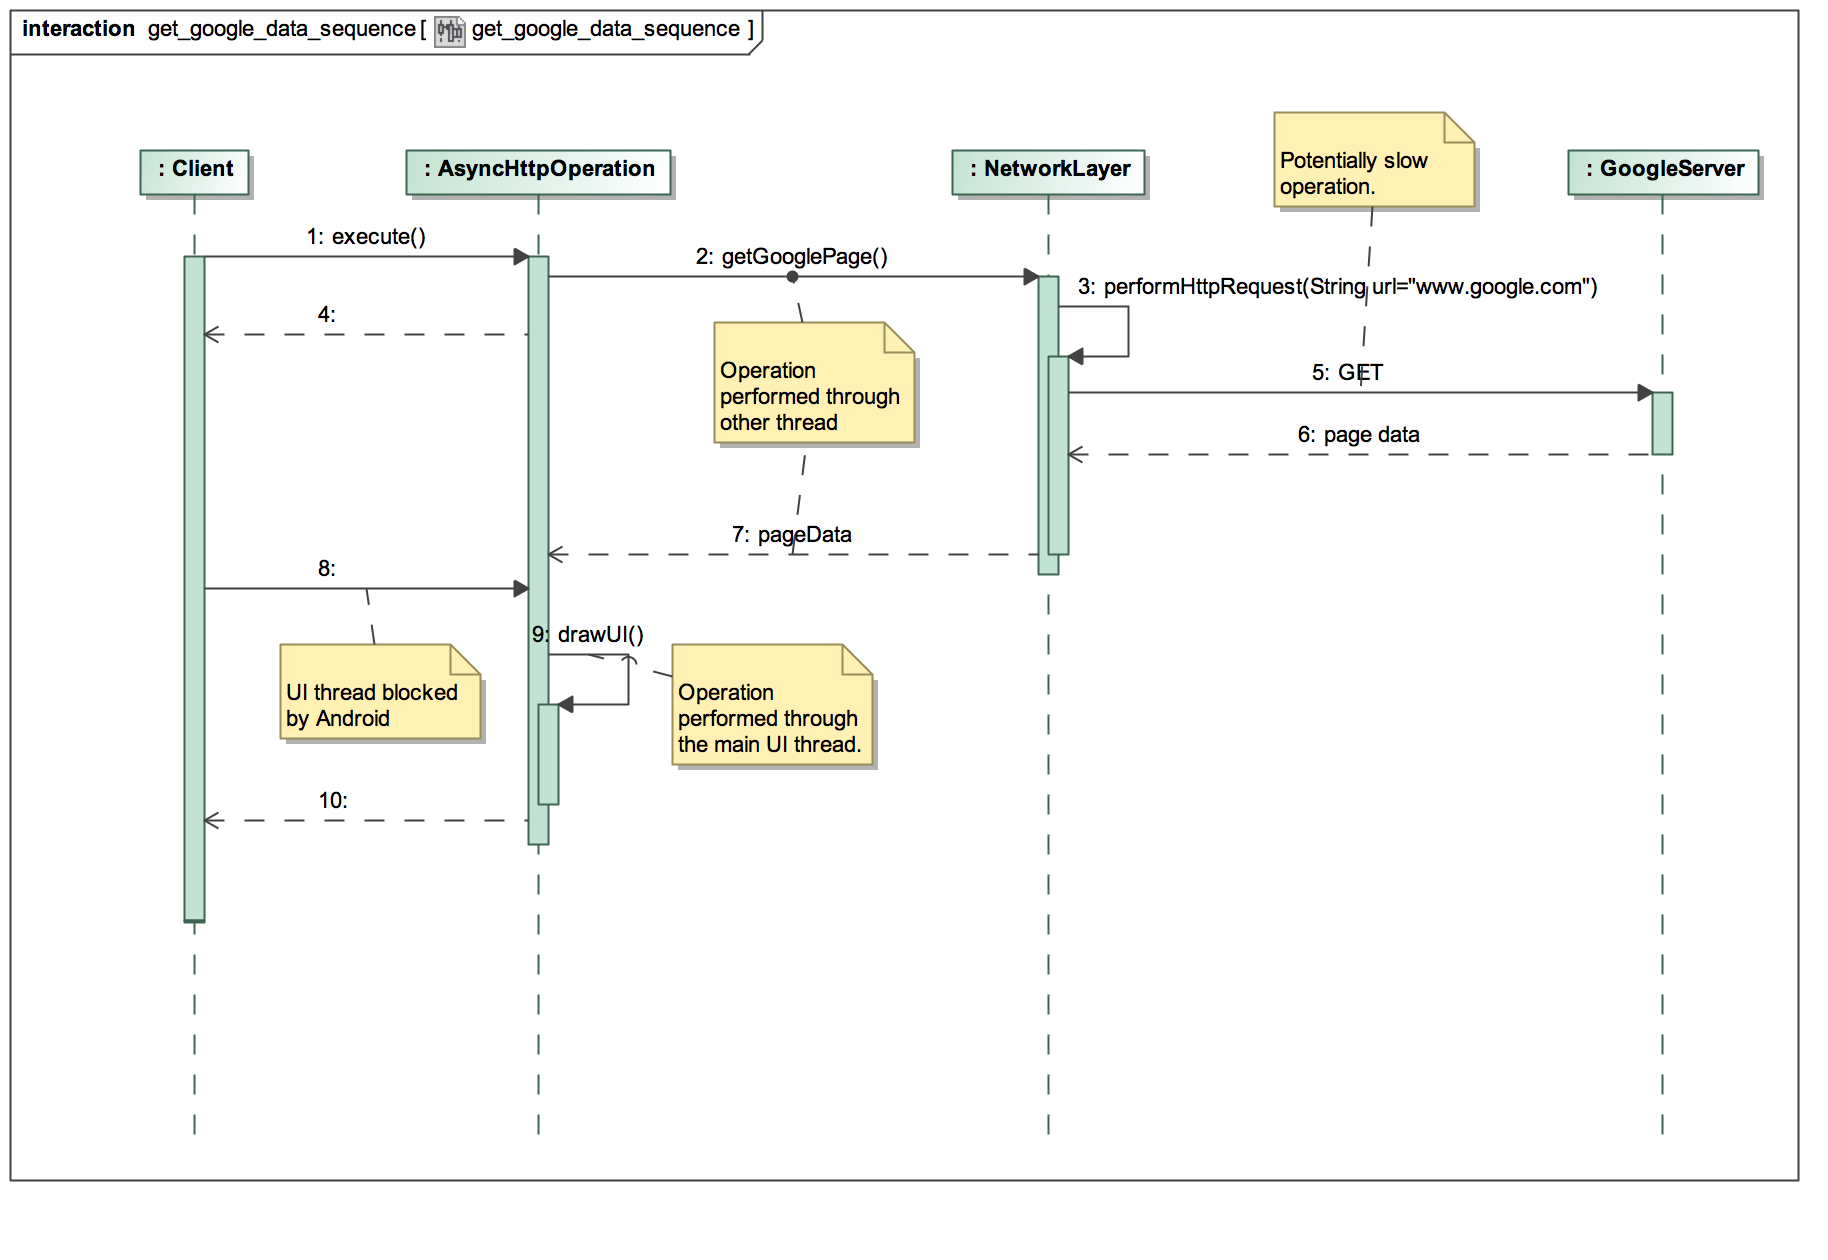
\includegraphics[scale=0.4]{../naive/design_models/get_google_data_sequence}
\end{center}
\end{figure}
\end{frame}

\begin{frame}{Explicación}
\begin{enumerate}
\item {\bf En el thread principal}: Cuando se llama a ``execute'' sobre la ``AsyncTask'' se devuelve el control inmediatamente.
\item {\bf Thread secundario}: Mientras tanto, se realiza la petición al servidor y se analiza la respuesta. 
\item {\bf Thread principal}: Una vez acabado el trabajo en segundo plano, se vuelve a bloquear el thread principal y se realizan las acciones que se hayan indicado (por ejemplo, mostrar un diálogo con el resultado de la respuesta).
\end{enumerate}
\begin{itemize}
\item {\bf Nota}: Mientras el thread secundario realiza la petición, el thread principal puede estar haciendo cualquier cosa (muchas veces se muestra un diálogo de carga, pero no siempre).
\end{itemize}
\end{frame}

\subsection{Conclusiones}
\begin{frame}{Conclusiones}
\begin{itemize}
\item Cada vez que se necesita hacer una petición (nueva o ya definida desde otra activity) y actualizar la interfaz, se define una clase que hereda de AsyncTask.
\item Es necesario definir la petición a realizar (clase ``NetworkOperationsManager''), el procesamiento de la respuesta y la actualización de la interfaz. Demasiadas responsabilidades.
\item Hay demasiado acoplamiento (se viola el SRP) $\rightarrow$ resulta dificultoso dividir la programación de la aplicación entre interfaz y bajo nivel (operaciones de red y cachés).
\end{itemize}
\end{frame}

\section{Segundo diseño: utilización de callbacks}
\subsection{Callbacks}
\begin{frame}{¿Qué es un callback?}
\begin{itemize}
\item Un callback es código ejecutable que se pasa como un argumento a otro código y se espera que sea llamado en un determinado momento.
\item Los callbacks pueden ser síncronos o asíncronos según se ejecuten de forma inmediata o no.
\item Los callbacks asíncronos exigen la existencia de más de un thread.
\item Pueden considerarse una forma de patrón Observador donde se le dice a una función que, cuando realize su tarea, ejecute la reacción de la entidad que la llama.
\end{itemize}
\end{frame}

\begin{frame}[fragile]{Ejemplo de callback: Lectura de un fichero en Node.js}
\begin{lstlisting}
fs = require('fs');
fs.readFile('path', 'utf8', function(err,data) {
  if (err) {
    return console.log(err);
  }
  console.log(data);
});
\end{lstlisting}


\end{frame}

\subsection{Diagrama de clases}
\begin{frame}
\begin{figure}
\begin{center}
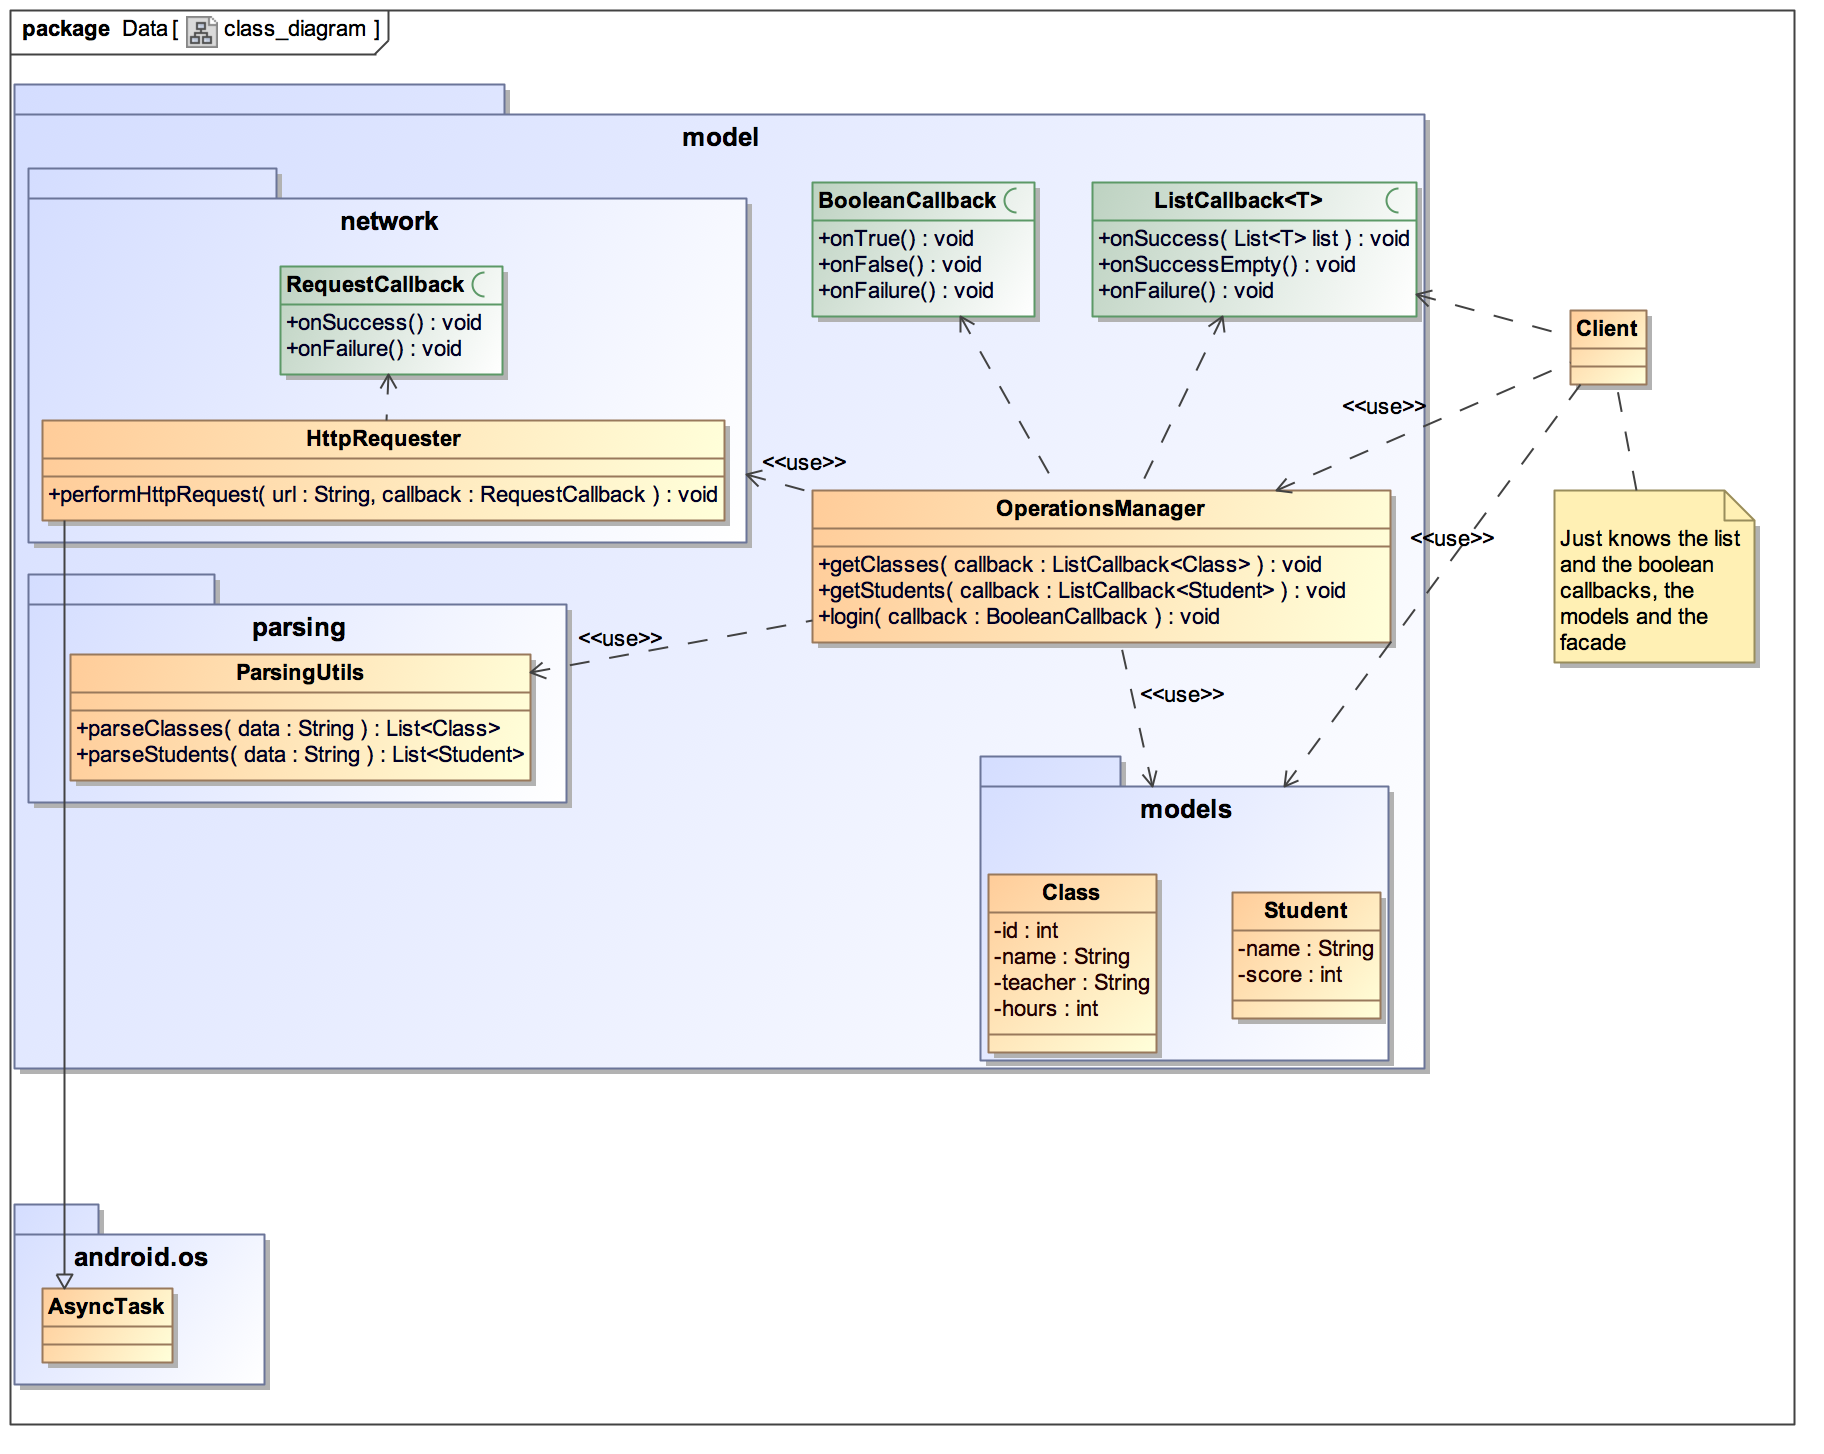
\includegraphics[scale=0.33]{../observer-pattern/diagrams/class_diagram}
\end{center}
\end{figure}
\end{frame}

\begin{frame}{Explicación (capa interna del modelo)}
\begin{itemize}
\item {\bf Network}: Este es el paquete más interno, define la acción básica de realizar una consulta HTTP y hacer ``algo'' con la respuesta. Ese ``algo'' se define mediante el ``RequestCallback''.
\item {\bf Parsing}: Funcionalidad relativa al ``parseo'' de las respuestas. 
\end{itemize} 
\end{frame}

\begin{frame}{Explicación (fachada del modelo)}
\begin{itemize}
\item {\bf OperationsManager}: Punto de entrada al subsistema, ofrece operaciones de red y requiere callbacks para saber qué hacer con las respuestas.
\item {\bf Callbacks}: Distintos tipos de callbacks que puedan requerir las operaciones del ``OperationsManager''.
\item {\bf Value\_objects}: Aquí van las clases que representan objetos (sin funcionalidad, equivalentes a las ``structs'' de C).
\end{itemize} 
\end{frame}

\subsection{Diagrama de secuencia}
\begin{frame}
\begin{figure}
\begin{center}
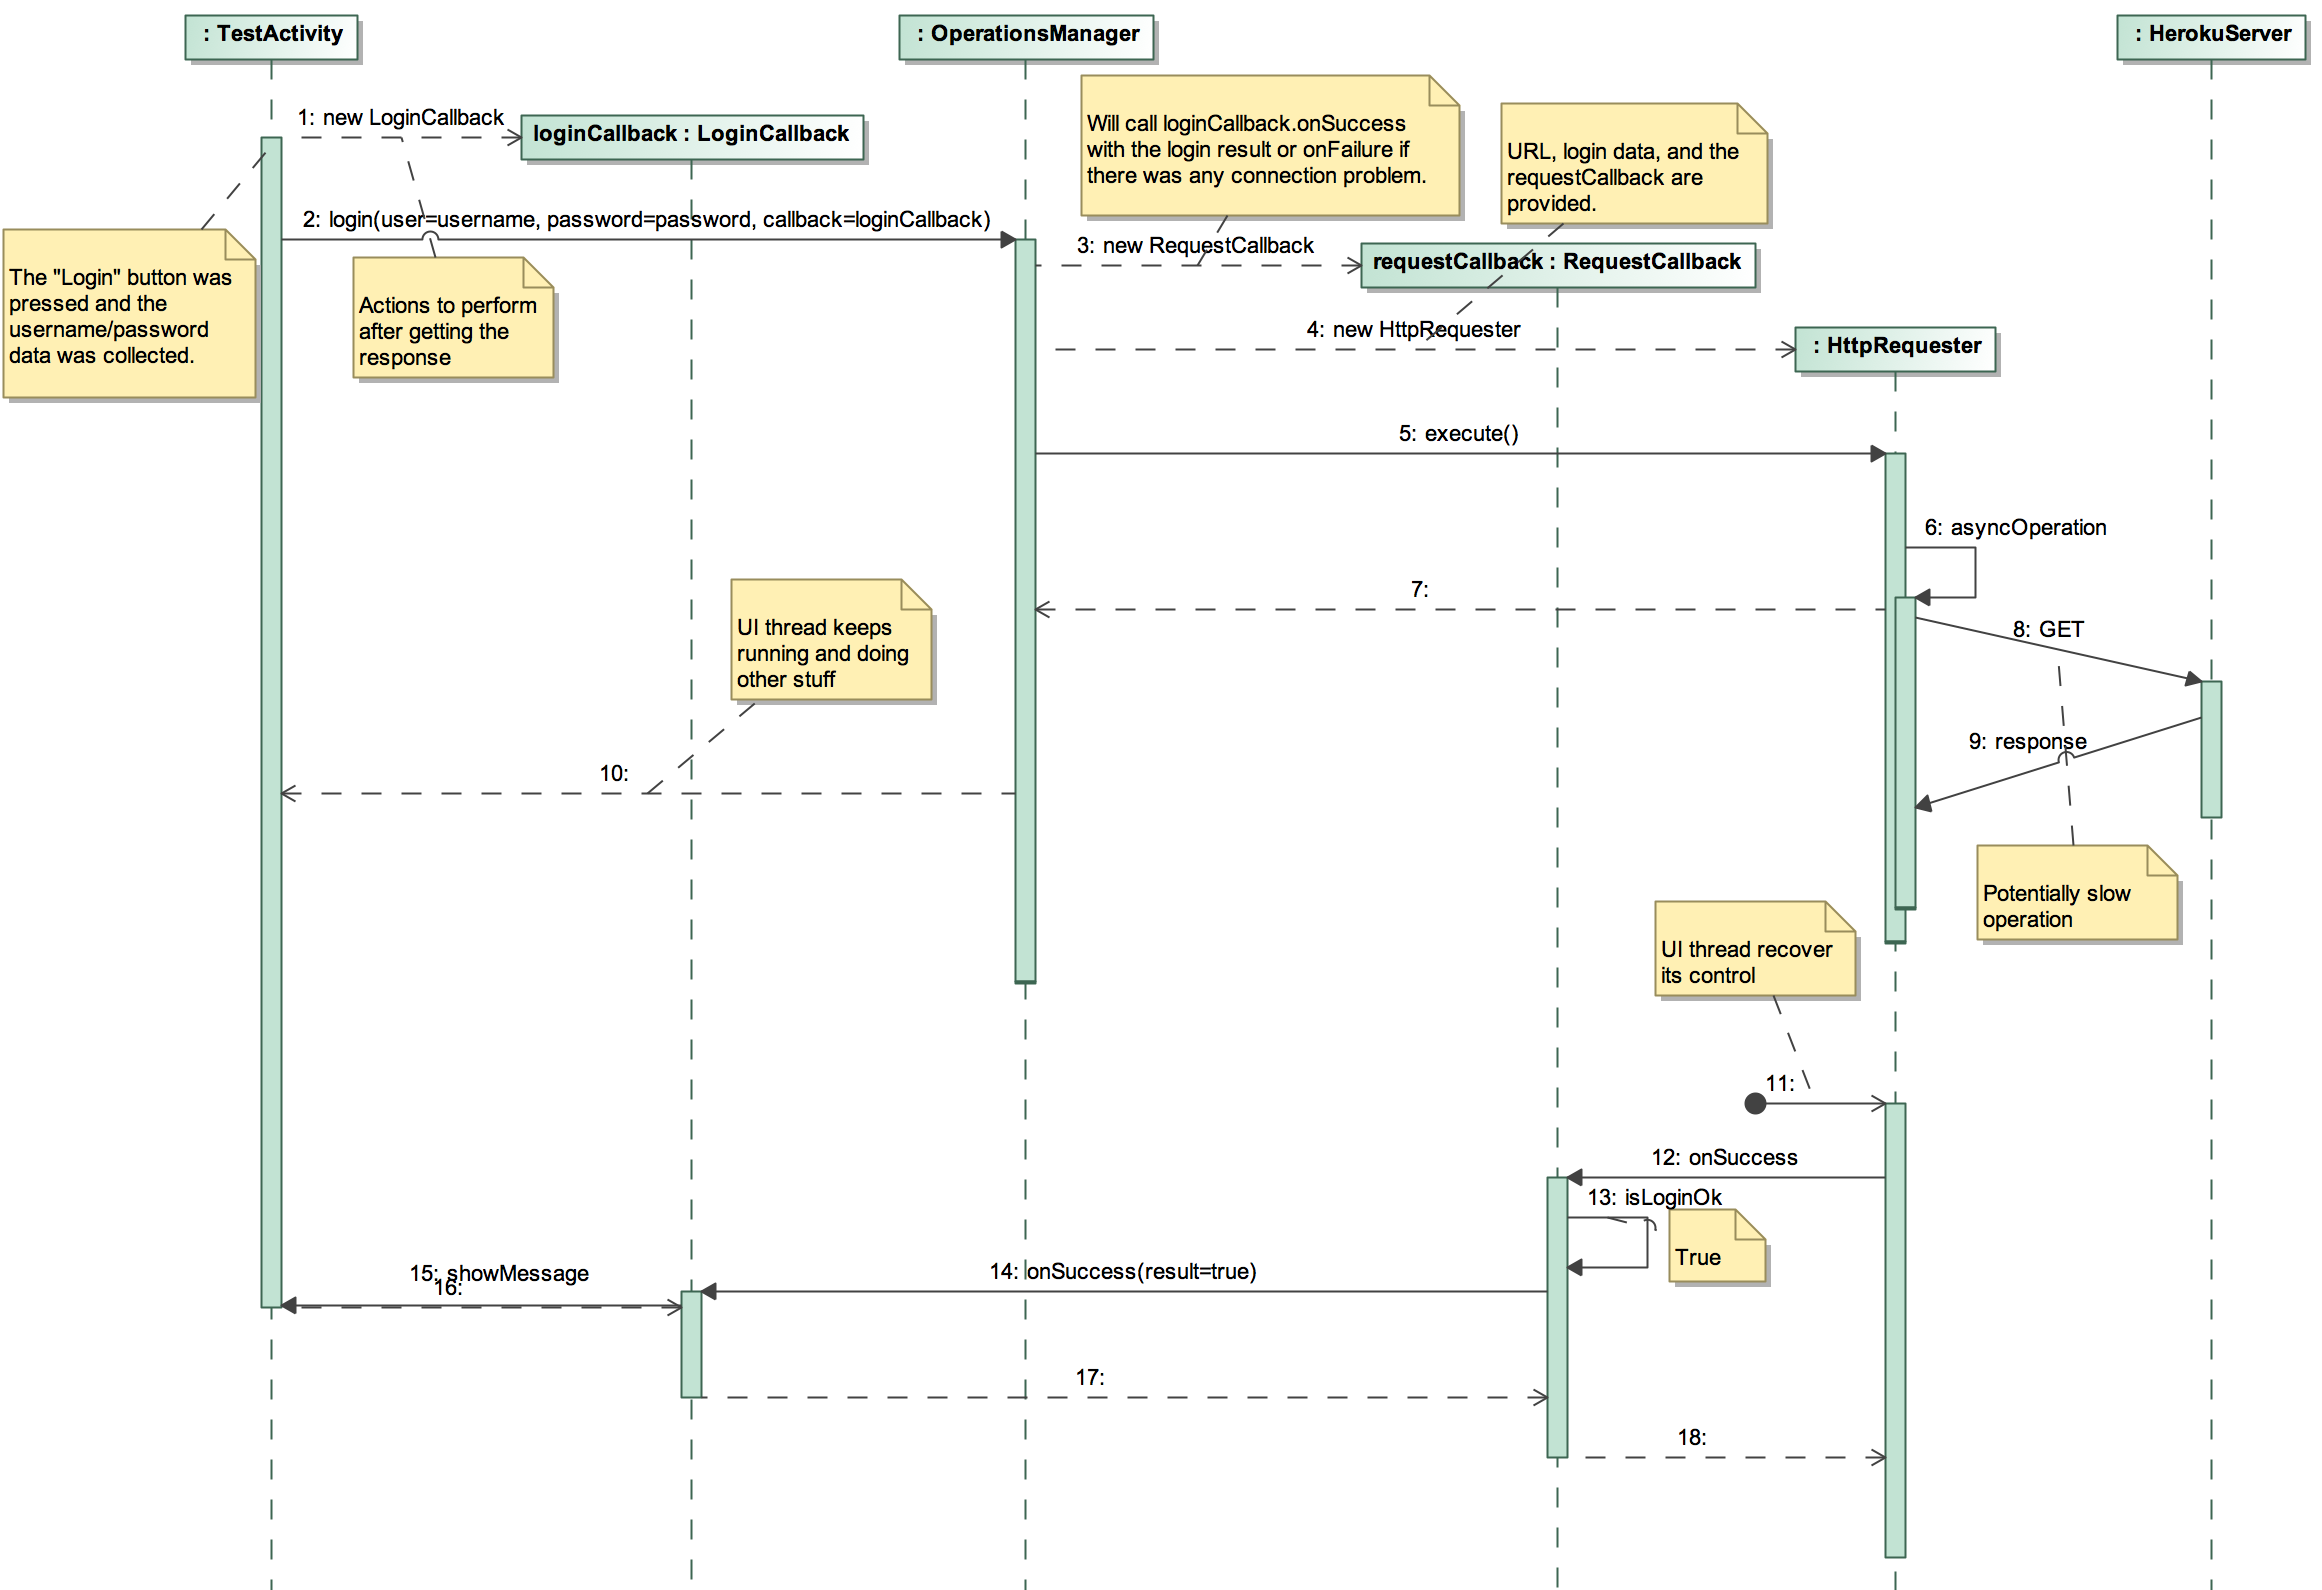
\includegraphics[scale=0.32]{../observer-pattern/diagrams/login}
\end{center}
\end{figure}
\end{frame}

\begin{frame}{Explicación}
\begin{enumerate}
\item Se crea un LoginCallback (esta clase implementa la interfaz OperationCallback con el tipo Boolean como parámetro)
\item Se llama a OperationsManager.getInstance().login(user, password, LoginCallback)
\item OperationsManager crea un RequestCallback y se lo manda al HttpRequester junto con la dirección y parámetros de la petición.
\item Aquí empieza la operación en segundo plano, mientras se devuelve el control de la interfaz.
\item Cuando la operación termina se ejecuta el código de RequestCallback, que a su vez llama a LoginCallback y realiza las operaciones pertinentes.
\end{enumerate} 
\end{frame}
\subsection{Conclusiones}
\begin{frame}[fragile]{Conclusiones}
\begin{itemize}
\item Esta aproximación se basa en tres conceptos: arquitectura MVC, patrón Observador (callbacks) y patrón Fachada.
\item {\bf Ventajas}:
\begin{itemize}

\item Las responsabilidades están claramente separadas.
\item El cliente del módulo de red solo necesita conocer la fachada.
\item Esta aproximación permite dividir la programación de interfaz y red completamente. Conectarlas es inmediato.
\end{itemize}

\item {\bf Limitaciones}: 
\begin{itemize}
\item Hay cierta repetición de código al no poder generalizar métodos como ``onFailure()''. \item La alternativa es utilizar una clase abstracta (pero no podriamos benificiarnos de implementar la interfaz directamente en una ``Activity'' si fuese lo suficientemente sencilla).
\end{itemize}
\end{itemize}
\end{frame}
\section{Extras}
\begin{frame}{Comentarios}
\begin{itemize}
\item El módulo más interno es común a un sinfín de aplicaciones Android $\rightarrow$ Convertirlo en una librería.
\item Alguien ha tenido la idea antes y ha hecho un muy buen trabajo: {\url http://loopj.com/android-async-http/}
\item Este mismo diseño puede ser aplicado a cualquier otra aplicación Java (u otra plataforma) siempre y cuando se implemente un mecanismo similar al AsyncTask (muchas plataformas no requieren actualizar la interfaz desde el thread principal).
\end{itemize}
\end{frame}

\begin{frame}{Repositorio}
\begin{itemize}
\item Diseño e implementación publicados en GitHub.
\item {\url https://github.com/SantiMunin/android-observer-pattern-example}
\end{itemize}
\end{frame}
\end{document}
